% Defense in depth: what stands between a proposed tool call and the host,
% and what verification does and does not prove. Built by make figures into
% pipeline.pdf (report, \textwidth) and docs/figures/pipeline.{svg,png}.
\pdfinfoomitdate=1
\pdftrailerid{}
\pdfsuppressptexinfo=-1
\documentclass[border=0pt]{standalone}
\usepackage{mathptmx}
\usepackage{courier}
\usepackage{tikz}
\usetikzlibrary{arrows.meta,calc,positioning}
% Shared look of the report figures: Times and Courier like the report body,
% a colour-blind-safe palette, thin dark lines.
\definecolor{statefill}{HTML}{E8EEF7}
\definecolor{verifyfill}{HTML}{DCE9F5}
\definecolor{replanfill}{HTML}{FFF2CC}
\definecolor{okfill}{HTML}{DFF0E0}
\definecolor{badfill}{HTML}{F8DEDE}
\definecolor{rejectcol}{HTML}{4477AA}
\definecolor{containcol}{HTML}{66CCEE}
\definecolor{residualcol}{HTML}{EE6677}
\definecolor{breachcol}{HTML}{222222}
\definecolor{inkcol}{HTML}{333333}
\tikzset{
  st/.style={draw=inkcol, rounded corners=2pt, fill=statefill, font=\small,
             minimum height=8mm, minimum width=16mm, inner sep=2pt},
  terminal/.style={st, double, double distance=1.2pt},
  edge/.style={-{Stealth[length=2.2mm, width=1.6mm]}, semithick, draw=inkcol},
  halo/.style={preaction={draw, white, line width=3.2pt, -}},
  lab/.style={font=\scriptsize, fill=white, inner sep=1pt, text=inkcol},
  note/.style={draw=inkcol!60, dashed, rounded corners=2pt, fill=white,
               font=\scriptsize, align=left, inner sep=3pt, text=inkcol},
  notelink/.style={dashed, draw=inkcol!60},
}

\tikzset{
  box/.style={draw=inkcol, rounded corners=2pt, fill=statefill, font=\footnotesize,
              align=center, inner sep=3pt, minimum height=12mm,
              execute at begin node={\hyphenpenalty=10000\exhyphenpenalty=10000}},
  check/.style={box, text width=3.0cm},
  head/.style={font=\small\bfseries},
}
\begin{document}
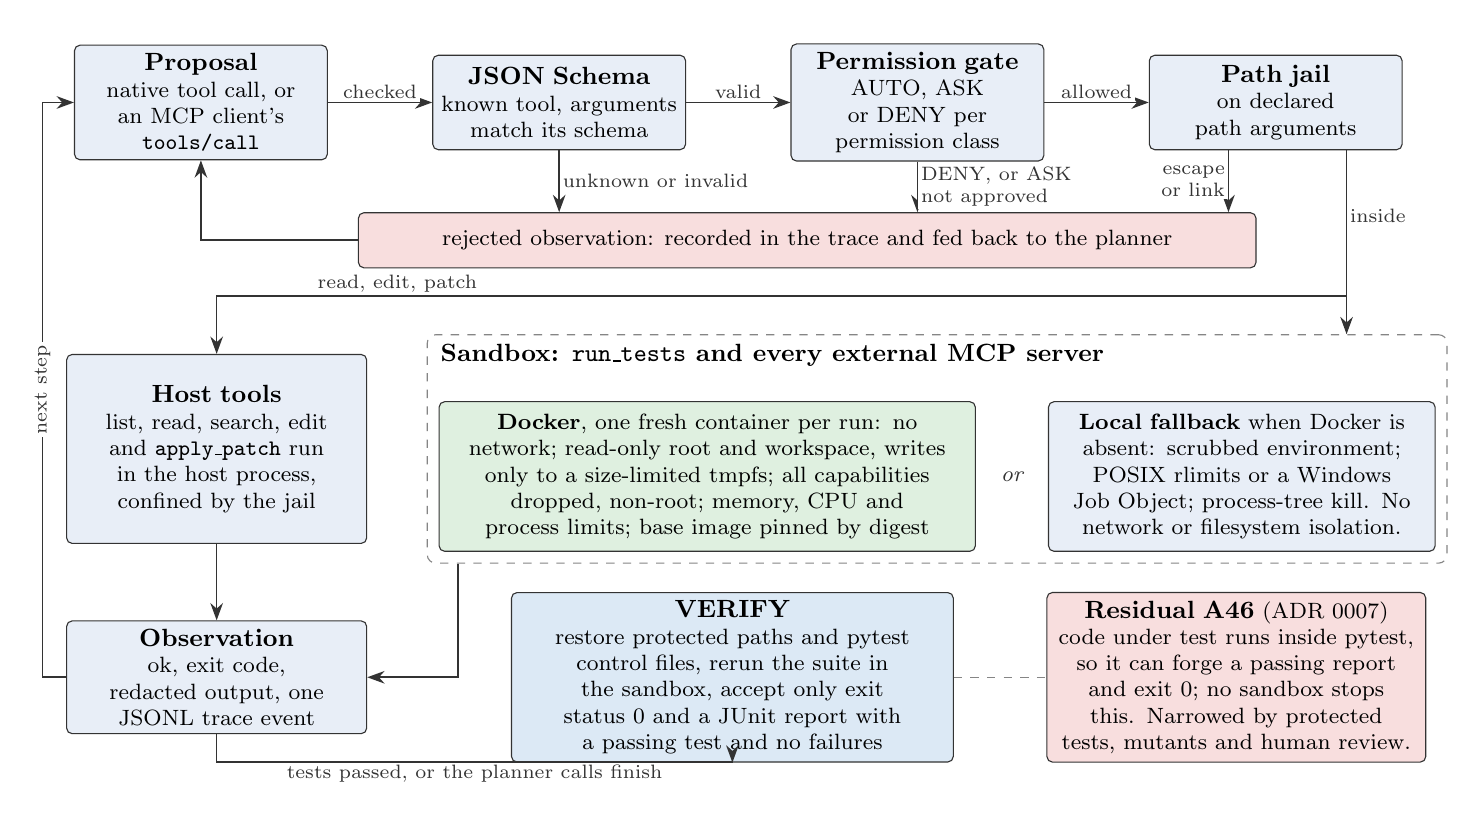
\begin{tikzpicture}[x=1cm, y=1cm]
% Exactly the report's \textwidth (516pt), opaque white.
\fill[white, use as bounding box] (0,-8.80) rectangle (516pt,0.95);

% Row 1: the checks every proposed call passes, in order.
\node[check] (prop) at (2.20,0)
  {{\small\bfseries Proposal}\\ native tool call, or an MCP client's \texttt{tools/call}};
\node[check] (schema) at (6.75,0)
  {{\small\bfseries JSON Schema}\\ known tool, arguments match its schema};
\node[check] (perm) at (11.30,0)
  {{\small\bfseries Permission gate}\\ AUTO, ASK or DENY per permission class};
\node[check] (jail) at (15.85,0)
  {{\small\bfseries Path jail}\\ on declared path arguments};
\draw[edge] (prop) -- node[lab, above] {checked} (schema);
\draw[edge] (schema) -- node[lab, above] {valid} (perm);
\draw[edge] (perm) -- node[lab, above] {allowed} (jail);

% Rejections never reach execution; they come back as observations.
\node[box, fill=badfill, minimum height=7mm, minimum width=11.4cm] (rej) at (9.90,-1.75)
  {rejected observation: recorded in the trace and fed back to the planner};
\draw[edge] (schema.south) -- node[lab, right] {unknown or invalid} (schema.south |- rej.north);
\draw[edge] (perm.south) -- node[lab, right, align=left] {DENY, or ASK\\ not approved} (perm.south |- rej.north);
\draw[edge] ([xshift=-6mm]jail.south) -- node[lab, left, align=right] {escape\\ or link} ([xshift=-6mm]jail.south |- rej.north);
\draw[edge] (rej.west) -| (prop.south);

% Row 2: where an accepted call runs.
\node[box, text width=3.6cm, minimum height=24mm] (host) at (2.40,-4.40)
  {{\small\bfseries Host tools}\\ list, read, search, edit and \texttt{apply\_patch} run in the
   host process, confined by the jail};
\node[draw=inkcol!60, dashed, rounded corners=3pt, minimum width=12.95cm, minimum height=29mm]
  (sbx) at (11.55,-4.40) {};
\node[head, anchor=north west, inner sep=2pt] at ($(sbx.north west)+(0.1,-0.05)$)
  {Sandbox: \texttt{run\_tests} and every external MCP server};
\node[box, fill=okfill, text width=6.6cm, minimum height=19mm, anchor=south west] (docker) at ($(sbx.south west)+(0.15,0.15)$)
  {{\bfseries Docker}, one fresh container per run: no network; read-only root and
   workspace, writes only to a size-limited tmpfs; all capabilities dropped,
   non-root; memory, CPU and process limits; base image pinned by digest};
\node[box, text width=4.7cm, minimum height=19mm, anchor=south east] (local) at ($(sbx.south east)+(-0.15,0.15)$)
  {{\bfseries Local fallback} when Docker is absent: scrubbed environment; POSIX
   rlimits or a Windows Job Object; process-tree kill. No network or
   filesystem isolation.};
\node[font=\footnotesize\itshape, text=inkcol] at ($(docker.east)!0.5!(local.west)$) {or};

% The dispatch bus from the jail to both places.
\draw[semithick, draw=inkcol] ([xshift=9mm]jail.south) -- node[lab, right, pos=0.45] {inside} ++(0,-1.85) coordinate (bus);
\draw[edge] (bus) -- (bus |- sbx.north);
\draw[edge] (bus) -| node[lab, pos=0.42, above] {read, edit, patch} (host.north);

% Row 3: observation, verification, and the residual it cannot close.
\node[box, text width=3.6cm] (obs) at (2.40,-7.30)
  {{\small\bfseries Observation}\\ ok, exit code, redacted output, one JSONL trace event};
\draw[edge] (host) -- (obs);
\draw[edge] ([xshift=4mm]sbx.south west) |- (obs.east);
\draw[edge] (obs.west) -- ++(-0.3,0) |- node[lab, pos=0.25, rotate=90] {next step} (prop.west);

\node[box, fill=verifyfill, text width=5.4cm] (verify) at (8.95,-7.30)
  {{\small\bfseries VERIFY}\\ restore protected paths and pytest control files,
   rerun the suite in the sandbox, accept only exit status 0 and a JUnit report
   with a passing test and no failures};
\draw[edge] (obs.south) -- ++(0,-0.35) -| node[lab, pos=0.25, below] {tests passed, or the planner calls finish} (verify.south);

\node[box, fill=badfill, text width=4.6cm] (a46) at (15.35,-7.30)
  {{\small\bfseries Residual A46} (ADR 0007)\\ code under test runs inside pytest,
   so it can forge a passing report and exit 0; no sandbox stops this.
   Narrowed by protected tests, mutants and human review.};
\draw[notelink] (verify.east) -- (a46.west);
\end{tikzpicture}
\end{document}
